\subsubsection{Modification Latency}

We now study  modification operations. As before, we experiment with bursts of rules. Modification latency is defined similar to insertion.

\minisection{\bf Table occupancy} To study the impact of table
occupancy, we pre-insert $S$ rules into a switch,
%(simple rules as before),
all with the same priority. We then modify one rule at a time by changing the
rule's output port, sending modification requests back to back. 

\begin{figure}[!tb]
\centering
\subfloat[100 rules in table \label{fig:bcm_mod_same_burst_100}]
  {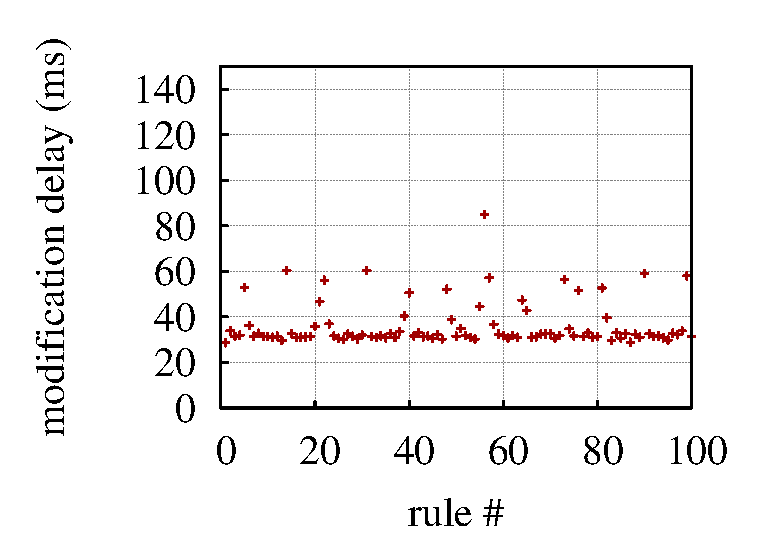
\includegraphics[width=.5\linewidth]{./figs/jan27_bcm_mod_same_burst_100_imc.eps}}\hfill
%\subfloat[burst size 100, increasing priority.\label{fig:bcm_mod_incr_burst_100}]
%  {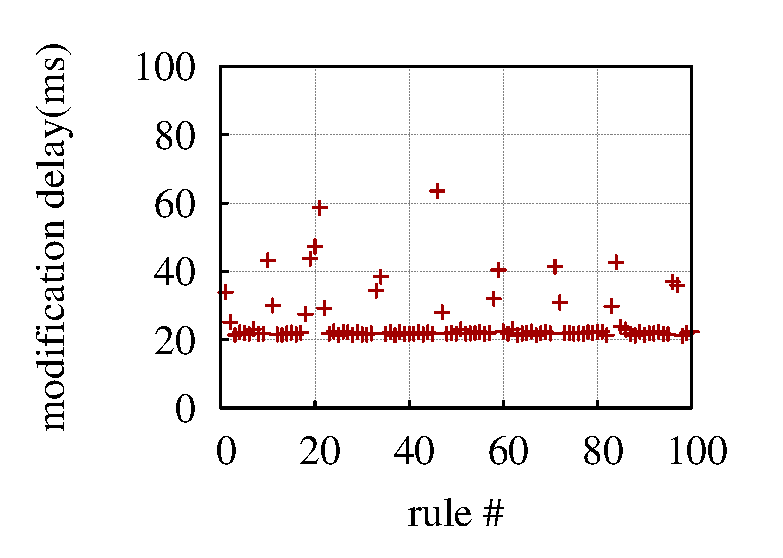
\includegraphics[width=.24\linewidth]{./figs/jan27_bcm_mod_incr_burst_100.eps}}\hfill
%\subfloat[burst size 100, decreasing priority.\label{fig:bcm_mod_decr_burst_100}]
%  {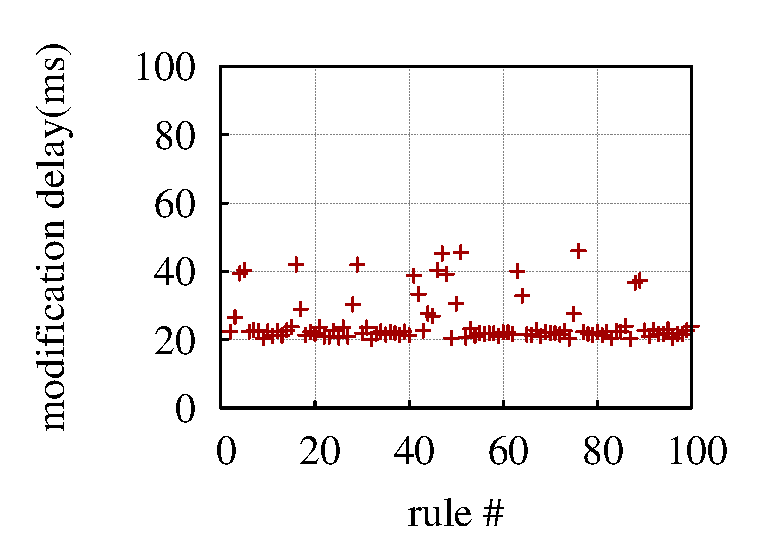
\includegraphics[width=.24\linewidth]{./figs/jan27_bcm_mod_decr_burst_100.eps}}\hfill
\subfloat[200 rules in table \label{fig:bcm_mod_same_burst_200}]
  {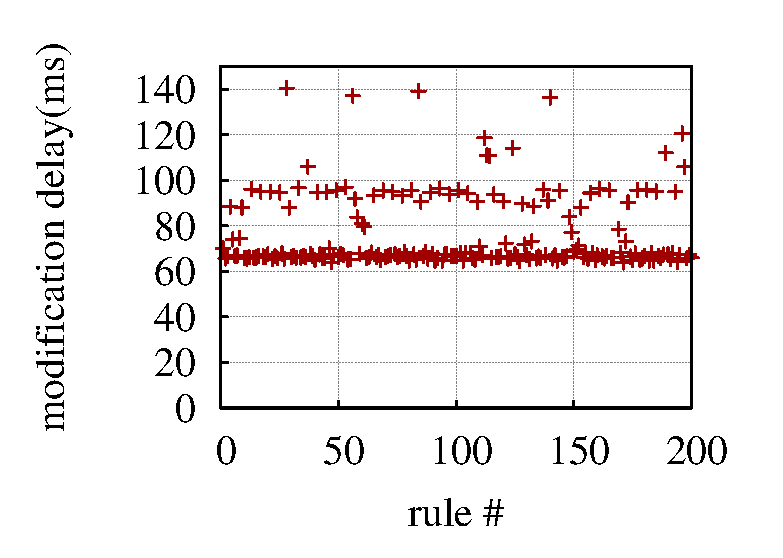
\includegraphics[width=.5\linewidth]{./figs/jan27_bcm_mod_same_burst_200.eps}}
\compactcaption{{\bf \BroadcomOne} per-rule {\bf mod.} latency, same priority}
\label{fig:occupancy-broadcom-modify}
\end{figure}
 
Per-rule modification delay for \BroadcomOne when $S=100$ and $S=200$ are shown in
\figsref{fig:bcm_mod_same_burst_100}{fig:bcm_mod_same_burst_200}, respectively. We
see that the per-rule delay
is more than 30 ms for $S=100$. When we double the number of rules,
$S=200$, latency doubles as well. It grows
linearly with $S$ (not shown). Note that
this latency is much higher than the corresponding
insertion latency (3.12ms per rule) (\S\ref{s:meas_insert}).
%\fixme{IBM added}
\IBM's per-rule modification latency is also affected significantly by the table occupancy---
the per-rule modification latencies for $S=100$ and $S=200$ are 18.77ms and 37.13ms, respectively.
 
\iffalse
\begin{figure}[!tb]
  \centering \subfloat[100 rules in table \label{fig:intel_mod_same_burst_100}]
  {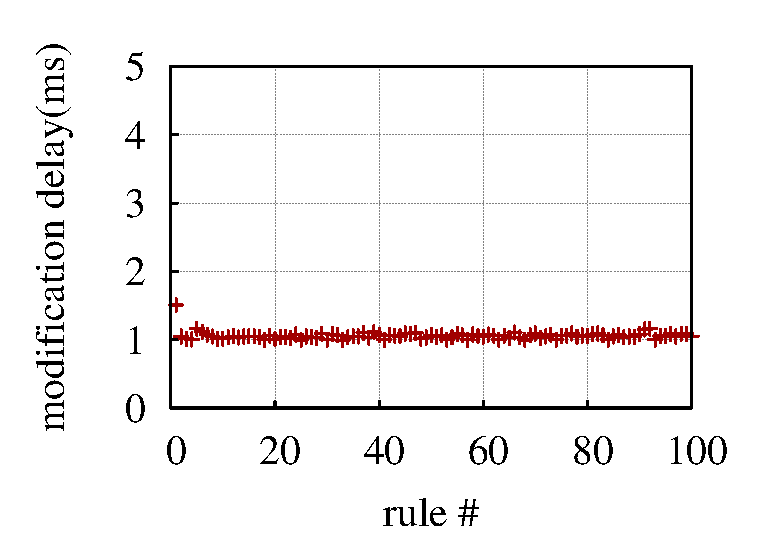
\includegraphics[width=.5\linewidth]{./figs/jan27_intel_mod_same_burst_100.eps}}\hfill
%\subfloat[burst size 100, increasing priority.\label{fig:intel_mod_incr_burst_100}]
%  {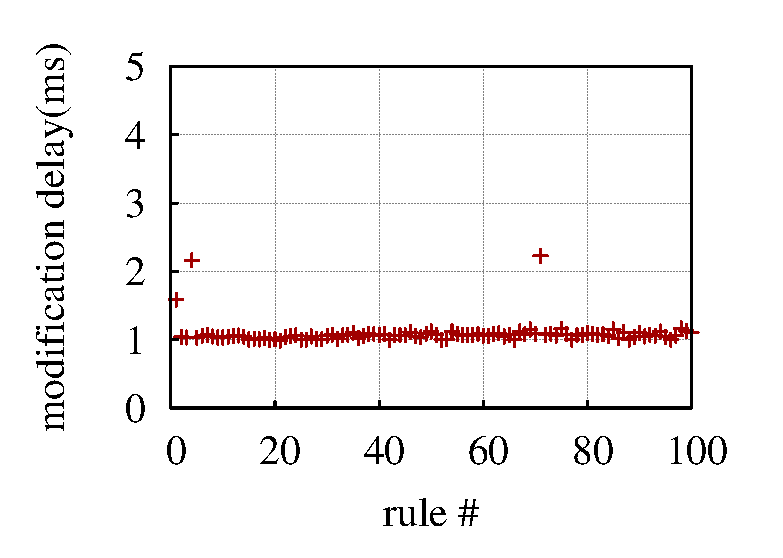
\includegraphics[width=.24\linewidth]{./figs/jan27_intel_mod_incr_burst_100.eps}}\hfill
%\subfloat[burst size 100, decreasing priority.\label{fig:intel_mod_decr_burst_100}]
%  {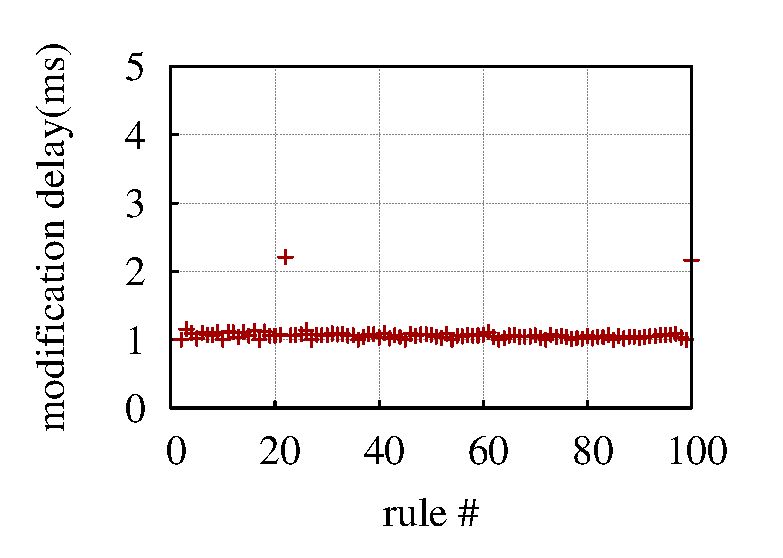
\includegraphics[width=.24\linewidth]{./figs/jan27_intel_mod_decr_burst_100.eps}}\hfill
\subfloat[200 rules in table \label{fig:intel_mod_same_burst_200}]
  {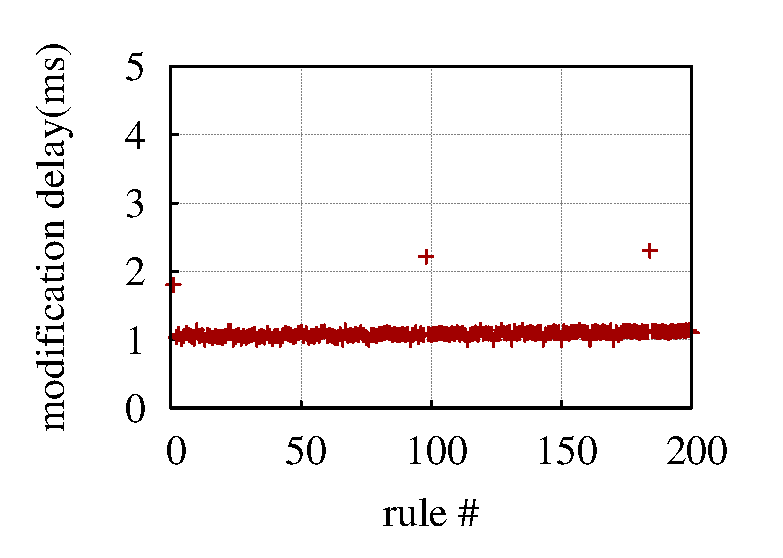
\includegraphics[width=.5\linewidth]{./figs/jan27_intel_mod_same_burst_200.eps}}
\compactcaption{{\bf \Intel} per-rule {\bf mod.} latency, same priority}
\label{fig:occupancy-intel-modify}
\end{figure}
\fi
%The results for $S=100,200$ for Intel are shown in
%Figure~\ref{fig:occupancy-intel-modify}. 
%Sourav commented
%For Intel, the modification delay for $S=100,200$ is around 1 ms
%(standard deviation 0.06) for all modified rules, similar to insertion
%in Figure~\ref{fig:priority-intel-insert}.
%delay with same priority,  in contrast with
%\BroadcomOne. 
% the modification delay is around 1 ms, which is the same as
% the insertion delay when all rules have same priority
% (\S\ref{s:meas_insert}).
% The results are the same for higher values of
% $S$.

In contrast, \Intel and \BroadcomThree  have lower modification delay,
and it does not vary with table occupancy. For \Intel (\BroadcomThree) the
per-rule modification delay for both $S=100$ and $S=200$ is around 1 ms (2ms)
for all modified rules, similar to (2X more than) same priority insertion delay. 

%\aditya{I changed the previous sentences. Check!!}
%%  For \BroadcomThree the average modification delay (standard deviation) for $S=100$ and $S=200$ is 2.19 (1.82) and 2.95 (2.29) respectively.
%For \BroadcomThree the modification delay is highly variable and is 
%related with table occupancy. For example, modifying 200 %rules in a table with 200 and 500 rules takes 449 and %4984 msec respectively. 

\minisection{Rule Priority} We conduct two experiments on each switch to
study the impact of rule priority. In
each experiment, we insert $B$ rules into an empty table ($S = 0$). In the 
{\em increasing} priority experiments, the rules in the table each have a
unique priority, and we send back-to-back modification requests for
rules in increasing priority order. We do the opposite in the {\em
decreasing priority} experiment. We vary $B$.%  across
% experiments. Note that the {\em same priority} experiment here is
% exactly the same as the table occupancy experiment above; hence we
% omit it.

\begin{figure}[!tb]
\centering
%\subfloat[burst size 100, same priority.\label{fig:bcm_mod_same_burst_100}]
%  {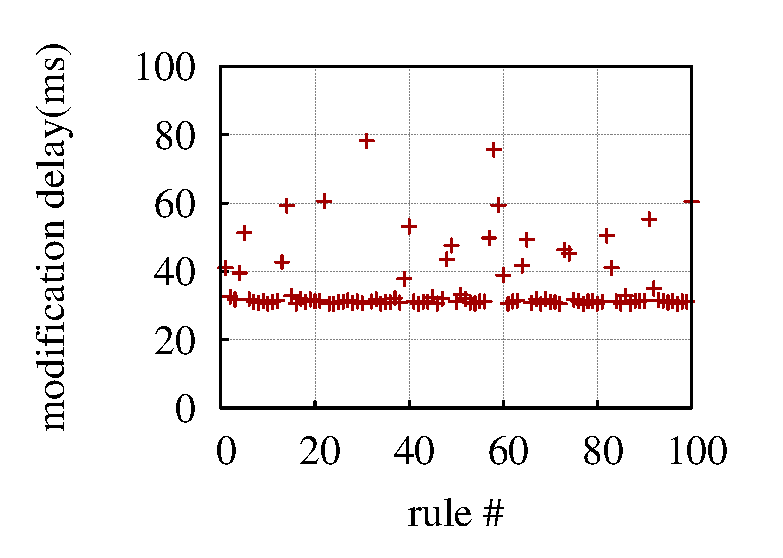
\includegraphics[width=.5\linewidth]{./figs/jan27_bcm_mod_same_burst_100.eps}}\hfill
\subfloat[burst size 100, incr. priority\label{fig:bcm_mod_incr_burst_100}]
  {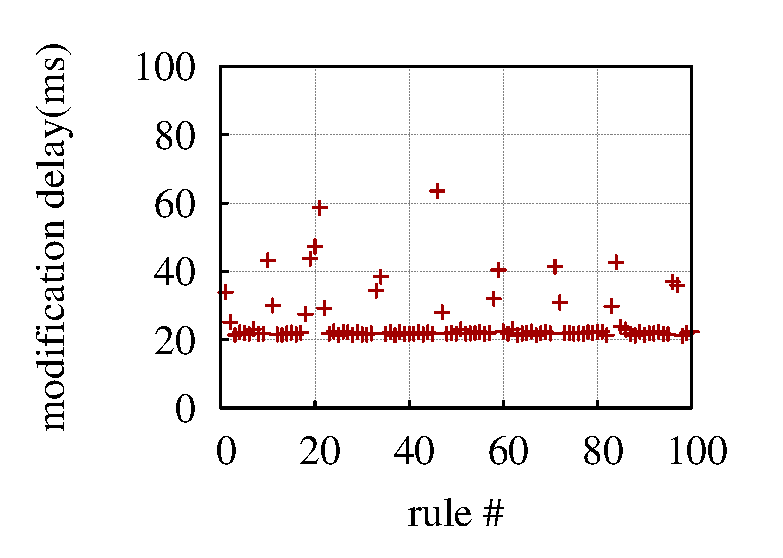
\includegraphics[width=.5\linewidth]{./figs/jan27_bcm_mod_incr_burst_100.eps}}\hfill
\subfloat[burst size 100, decr. priority\label{fig:bcm_mod_decr_burst_100}]
  {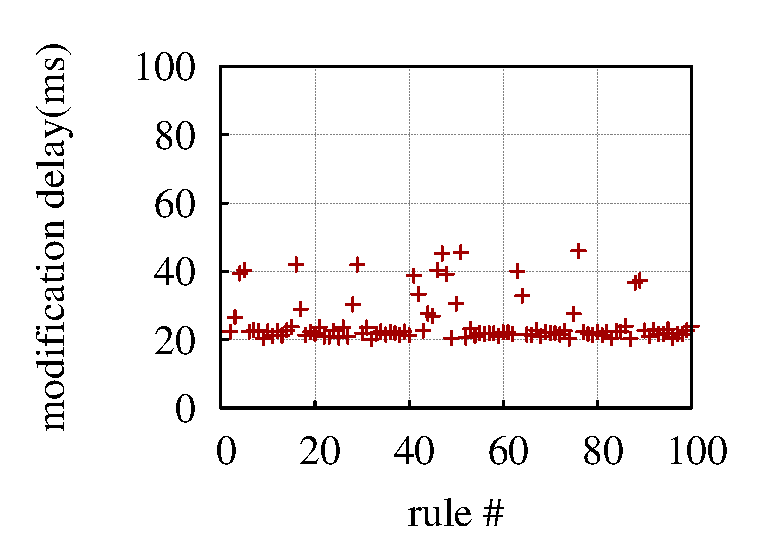
\includegraphics[width=.5\linewidth]{./figs/jan27_bcm_mod_decr_burst_100.eps}}\hfill
%\subfloat[burst size 200, same priority.\label{fig:bcm_mod_same_burst_200}]
%  {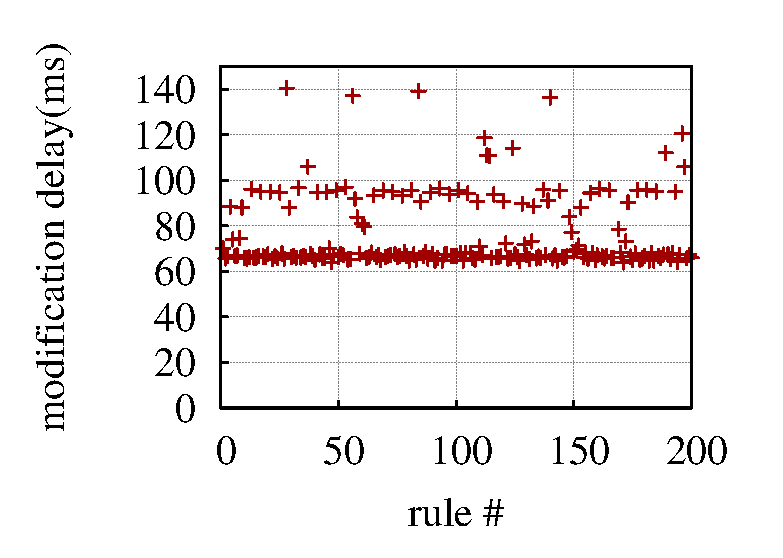
\includegraphics[width=.5\linewidth]{./figs/jan27_bcm_mod_same_burst_200.eps}}
\compactcaption{{\bf \BroadcomOne} priority per-rule {\bf modification} latency}
\label{fig:priority-broadcom-modify}
\end{figure}

%\emph{\BroadcomOne: increasing/decreasing priority.}
\figsref{fig:bcm_mod_incr_burst_100}{fig:bcm_mod_decr_burst_100} show the results for the increasing and decreasing priority experiments, respectively, for
$B=100$ on \BroadcomOne. In both cases, we see: (1) the per-rule modification delay is similar
across the rules, with a median of 25.10ms and a standard deviation of
6.74ms, and (2) the latencies are identical across the experiments. 
We similarly observe that priority does not affect modification delay in
\BroadcomThree, \Intel and \IBM (not shown).
% Again, the
% latencies are  much larger than insertion with same priority, 25 ms vs 3 ms.
%\aditya{this is not true! bcm insertion latencies are also high!} 
%li: add same priority, fixed, right?
%We observed that the latencies grew with $B$ for both experiments.
% increasing and decreasing
% priority experiments.

% Figure~\ref{fig:priority-broadcom-modify}-d shows the results for
% $B=200$, and again the per rule latency is about twice as high as that
% for $B=100$. 
% % per-rule modification delay for 200 rules has a median 60 (xx) ms and
% % standard deviation xx. The modification time is significant impacted
% % by the number of rules in the table.

% \emph{Broadcom: decreasing priority.}  We modify in both increasing rule
%   priority and decreasing rule priority. As shown in
%   Figure~\ref{fig:priority-broadcom-insert}-b,c, the per rule modification delay
%   is not affected by rule priority. Their median delay is xx and xx respectively
%   with standard deviation xx and xx.

%We next describe our measurement results on Intel. 
\iffalse
\begin{figure}[!tb]
\centering
%\subfloat[burst size 100, same priority.\label{fig:intel_mod_same_burst_100}]
%  {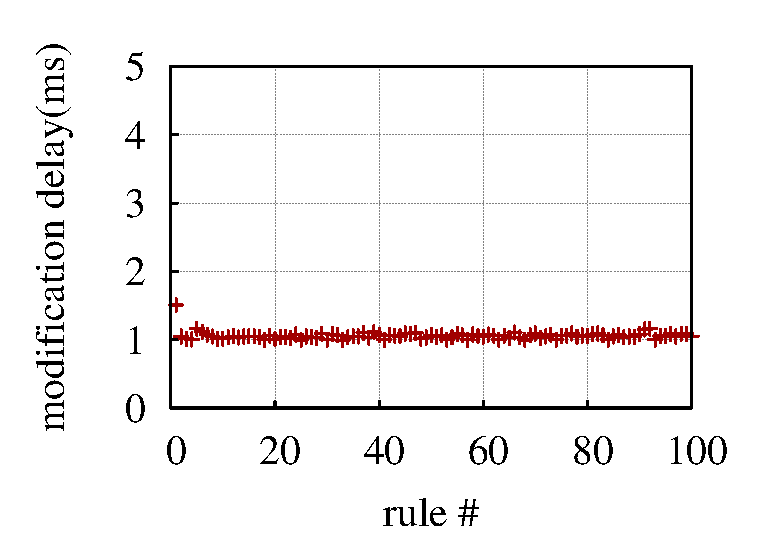
\includegraphics[width=.5\linewidth]{./figs/jan27_intel_mod_same_burst_100.eps}}\hfill
\subfloat[burst size 100, increasing priority.\label{fig:intel_mod_incr_burst_100}]
  {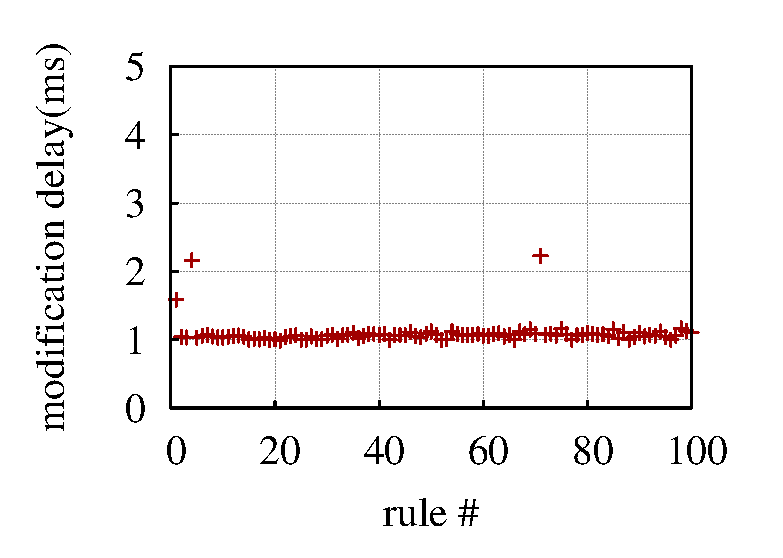
\includegraphics[width=.5\linewidth]{./figs/jan27_intel_mod_incr_burst_100.eps}}\hfill
 \subfloat[burst size 100, decreasing priority.\label{fig:intel_mod_decr_burst_100}]
  {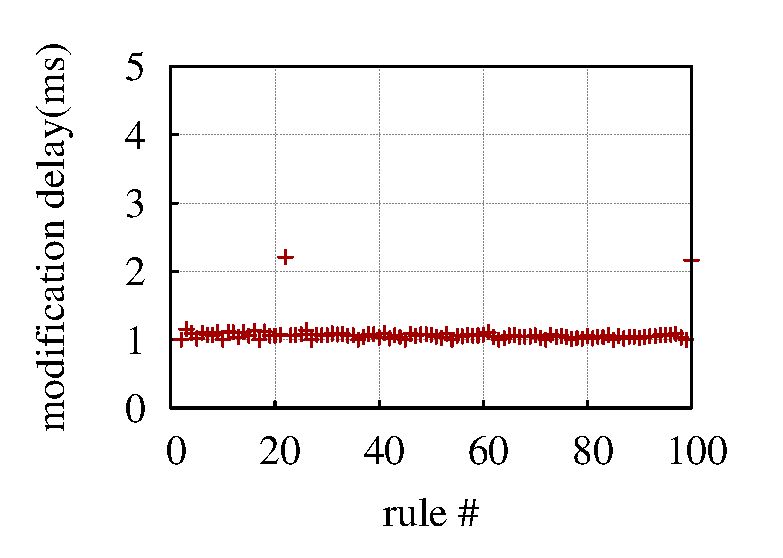
\includegraphics[width=.5\linewidth]{./figs/jan27_intel_mod_decr_burst_100.eps}}\hfill
%\subfloat[burst size 200, same priority.\label{fig:intel_mod_same_burst_200}]
%  {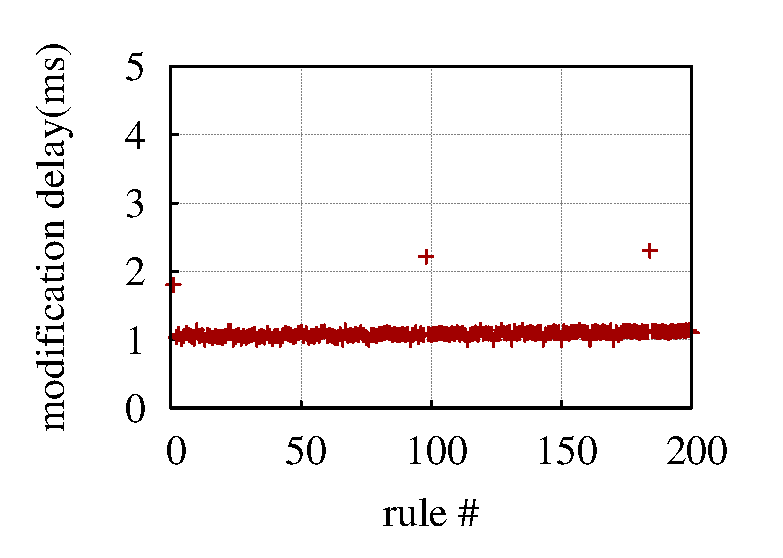
\includegraphics[width=.5\linewidth]{./figs/jan27_intel_mod_same_burst_200.eps}}
\caption{{\bf Intel} priority per-rule {\bf modification} latency results}
\label{fig:priority-intel-modify}
\end{figure}
\fi

%{\em Intel increasing/decreasing priority.} 
%Figure~\ref{fig:priority-intel-modify} shows the result for $B=100$ on
%Intel.
% , similar to insertion delay without
% priority.  We also tried other B values and the results are similar (omitted for brevity).


\minisection{Summary and root causes}
%Given our table occupancy and rule priority results, 
We conclude that the per-rule modification latency on \BroadcomOne and \IBM is 
impacted purely by table occupancy, not by rule priority structure.
For \BroadcomThree and \Intel, the per-rule modification delay 
%is 1 ms respectively 
is independent of rule priority, table occupancy, and burst size;
\BroadcomThree's per-rule modification delay is 2X higher than insertion.
%For \BroadcomThree, the modification delay is independent of rule priority but 
%is highly variable and is          
%related with table occupancy. The root cause of the variable and larger modification delay on 
%\BroadcomOne and \BroadcomThree is that modification involves insertion and deletion operation and it causes
%TCAM reorganization.

%We observe that flow rule priority do
%not impact modification delay. Modification delay in \BroadcomOne and \BroadcomThree is a
%function of table occupancy, whereas this is not the case for Intel where modification is as fast as insertion. 
Conversations with Broadcom indicated that TCAM modification should ideally be fast and independent of table size, 
so the underlying cause appears to be less optimized switch software in \BroadcomOne. Indeed, our measurements with \BroadcomThree show that this issue has (at least partly) been fixed.

% However, for Broadcom, the modification delay is much higher
% than rule insertion delay with same priority. For Intel, the modification delay
% is similar to rule insertion delay with same priority. 

% \aditya{missing causes!}


% LocalWords:  pre Broadcom
